% Options for packages loaded elsewhere
% Options for packages loaded elsewhere
\PassOptionsToPackage{unicode}{hyperref}
\PassOptionsToPackage{hyphens}{url}
\PassOptionsToPackage{dvipsnames,svgnames,x11names}{xcolor}
%
\documentclass[
  spanish,
  a4paper,
]{scrreport}
\usepackage{xcolor}
\usepackage{amsmath,amssymb}
\setcounter{secnumdepth}{5}
\usepackage{iftex}
\ifPDFTeX
  \usepackage[T1]{fontenc}
  \usepackage[utf8]{inputenc}
  \usepackage{textcomp} % provide euro and other symbols
\else % if luatex or xetex
  \usepackage{unicode-math} % this also loads fontspec
  \defaultfontfeatures{Scale=MatchLowercase}
  \defaultfontfeatures[\rmfamily]{Ligatures=TeX,Scale=1}
\fi
\usepackage{lmodern}
\ifPDFTeX\else
  % xetex/luatex font selection
\fi
% Use upquote if available, for straight quotes in verbatim environments
\IfFileExists{upquote.sty}{\usepackage{upquote}}{}
\IfFileExists{microtype.sty}{% use microtype if available
  \usepackage[]{microtype}
  \UseMicrotypeSet[protrusion]{basicmath} % disable protrusion for tt fonts
}{}
\makeatletter
\@ifundefined{KOMAClassName}{% if non-KOMA class
  \IfFileExists{parskip.sty}{%
    \usepackage{parskip}
  }{% else
    \setlength{\parindent}{0pt}
    \setlength{\parskip}{6pt plus 2pt minus 1pt}}
}{% if KOMA class
  \KOMAoptions{parskip=half}}
\makeatother
% Make \paragraph and \subparagraph free-standing
\makeatletter
\ifx\paragraph\undefined\else
  \let\oldparagraph\paragraph
  \renewcommand{\paragraph}{
    \@ifstar
      \xxxParagraphStar
      \xxxParagraphNoStar
  }
  \newcommand{\xxxParagraphStar}[1]{\oldparagraph*{#1}\mbox{}}
  \newcommand{\xxxParagraphNoStar}[1]{\oldparagraph{#1}\mbox{}}
\fi
\ifx\subparagraph\undefined\else
  \let\oldsubparagraph\subparagraph
  \renewcommand{\subparagraph}{
    \@ifstar
      \xxxSubParagraphStar
      \xxxSubParagraphNoStar
  }
  \newcommand{\xxxSubParagraphStar}[1]{\oldsubparagraph*{#1}\mbox{}}
  \newcommand{\xxxSubParagraphNoStar}[1]{\oldsubparagraph{#1}\mbox{}}
\fi
\makeatother

\usepackage{color}
\usepackage{fancyvrb}
\newcommand{\VerbBar}{|}
\newcommand{\VERB}{\Verb[commandchars=\\\{\}]}
\DefineVerbatimEnvironment{Highlighting}{Verbatim}{commandchars=\\\{\}}
% Add ',fontsize=\small' for more characters per line
\usepackage{framed}
\definecolor{shadecolor}{RGB}{241,243,245}
\newenvironment{Shaded}{\begin{snugshade}}{\end{snugshade}}
\newcommand{\AlertTok}[1]{\textcolor[rgb]{0.68,0.00,0.00}{#1}}
\newcommand{\AnnotationTok}[1]{\textcolor[rgb]{0.37,0.37,0.37}{#1}}
\newcommand{\AttributeTok}[1]{\textcolor[rgb]{0.40,0.45,0.13}{#1}}
\newcommand{\BaseNTok}[1]{\textcolor[rgb]{0.68,0.00,0.00}{#1}}
\newcommand{\BuiltInTok}[1]{\textcolor[rgb]{0.00,0.23,0.31}{#1}}
\newcommand{\CharTok}[1]{\textcolor[rgb]{0.13,0.47,0.30}{#1}}
\newcommand{\CommentTok}[1]{\textcolor[rgb]{0.37,0.37,0.37}{#1}}
\newcommand{\CommentVarTok}[1]{\textcolor[rgb]{0.37,0.37,0.37}{\textit{#1}}}
\newcommand{\ConstantTok}[1]{\textcolor[rgb]{0.56,0.35,0.01}{#1}}
\newcommand{\ControlFlowTok}[1]{\textcolor[rgb]{0.00,0.23,0.31}{\textbf{#1}}}
\newcommand{\DataTypeTok}[1]{\textcolor[rgb]{0.68,0.00,0.00}{#1}}
\newcommand{\DecValTok}[1]{\textcolor[rgb]{0.68,0.00,0.00}{#1}}
\newcommand{\DocumentationTok}[1]{\textcolor[rgb]{0.37,0.37,0.37}{\textit{#1}}}
\newcommand{\ErrorTok}[1]{\textcolor[rgb]{0.68,0.00,0.00}{#1}}
\newcommand{\ExtensionTok}[1]{\textcolor[rgb]{0.00,0.23,0.31}{#1}}
\newcommand{\FloatTok}[1]{\textcolor[rgb]{0.68,0.00,0.00}{#1}}
\newcommand{\FunctionTok}[1]{\textcolor[rgb]{0.28,0.35,0.67}{#1}}
\newcommand{\ImportTok}[1]{\textcolor[rgb]{0.00,0.46,0.62}{#1}}
\newcommand{\InformationTok}[1]{\textcolor[rgb]{0.37,0.37,0.37}{#1}}
\newcommand{\KeywordTok}[1]{\textcolor[rgb]{0.00,0.23,0.31}{\textbf{#1}}}
\newcommand{\NormalTok}[1]{\textcolor[rgb]{0.00,0.23,0.31}{#1}}
\newcommand{\OperatorTok}[1]{\textcolor[rgb]{0.37,0.37,0.37}{#1}}
\newcommand{\OtherTok}[1]{\textcolor[rgb]{0.00,0.23,0.31}{#1}}
\newcommand{\PreprocessorTok}[1]{\textcolor[rgb]{0.68,0.00,0.00}{#1}}
\newcommand{\RegionMarkerTok}[1]{\textcolor[rgb]{0.00,0.23,0.31}{#1}}
\newcommand{\SpecialCharTok}[1]{\textcolor[rgb]{0.37,0.37,0.37}{#1}}
\newcommand{\SpecialStringTok}[1]{\textcolor[rgb]{0.13,0.47,0.30}{#1}}
\newcommand{\StringTok}[1]{\textcolor[rgb]{0.13,0.47,0.30}{#1}}
\newcommand{\VariableTok}[1]{\textcolor[rgb]{0.07,0.07,0.07}{#1}}
\newcommand{\VerbatimStringTok}[1]{\textcolor[rgb]{0.13,0.47,0.30}{#1}}
\newcommand{\WarningTok}[1]{\textcolor[rgb]{0.37,0.37,0.37}{\textit{#1}}}

\usepackage{longtable,booktabs,array}
\newcounter{none} % for unnumbered tables
\usepackage{calc} % for calculating minipage widths
% Correct order of tables after \paragraph or \subparagraph
\usepackage{etoolbox}
\makeatletter
\patchcmd\longtable{\par}{\if@noskipsec\mbox{}\fi\par}{}{}
\makeatother
% Allow footnotes in longtable head/foot
\IfFileExists{footnotehyper.sty}{\usepackage{footnotehyper}}{\usepackage{footnote}}
\makesavenoteenv{longtable}
\usepackage{graphicx}
\makeatletter
\newsavebox\pandoc@box
\newcommand*\pandocbounded[1]{% scales image to fit in text height/width
  \sbox\pandoc@box{#1}%
  \Gscale@div\@tempa{\textheight}{\dimexpr\ht\pandoc@box+\dp\pandoc@box\relax}%
  \Gscale@div\@tempb{\linewidth}{\wd\pandoc@box}%
  \ifdim\@tempb\p@<\@tempa\p@\let\@tempa\@tempb\fi% select the smaller of both
  \ifdim\@tempa\p@<\p@\scalebox{\@tempa}{\usebox\pandoc@box}%
  \else\usebox{\pandoc@box}%
  \fi%
}
% Set default figure placement to htbp
\def\fps@figure{htbp}
\makeatother



\ifLuaTeX
\usepackage[bidi=basic,shorthands=off]{babel}
\else
\usepackage[bidi=default,shorthands=off]{babel}
\fi
\ifLuaTeX
  \usepackage{selnolig} % disable illegal ligatures
\fi


\setlength{\emergencystretch}{3em} % prevent overfull lines

\providecommand{\tightlist}{%
  \setlength{\itemsep}{0pt}\setlength{\parskip}{0pt}}



 


\usepackage{venndiagram}
\newcommand{\NN}{\mathbb{N}}
\newcommand{\ZZ}{\mathbb{Z}}
\newcommand{\QQ}{\mathbb{Q}}
\newcommand{\RR}{\mathbb{R}}
\newcommand{\CC}{\mathbb{C}}
\DeclareMathOperator{\operatorname{Int}}{Int}
\DeclareMathOperator{\operatorname{Ext}}{Ext}
\DeclareMathOperator{\operatorname{Fr}}{Fr}
\DeclareMathOperator{\Adh}{Adh}
\DeclareMathOperator{\Ac}{Ac}
\DeclareMathOperator{\sen}{sen}
\makeatletter
\@ifpackageloaded{tcolorbox}{}{\usepackage[skins,breakable]{tcolorbox}}
\@ifpackageloaded{fontawesome5}{}{\usepackage{fontawesome5}}
\definecolor{quarto-callout-color}{HTML}{909090}
\definecolor{quarto-callout-note-color}{HTML}{0758E5}
\definecolor{quarto-callout-important-color}{HTML}{CC1914}
\definecolor{quarto-callout-warning-color}{HTML}{EB9113}
\definecolor{quarto-callout-tip-color}{HTML}{00A047}
\definecolor{quarto-callout-caution-color}{HTML}{FC5300}
\definecolor{quarto-callout-color-frame}{HTML}{acacac}
\definecolor{quarto-callout-note-color-frame}{HTML}{4582ec}
\definecolor{quarto-callout-important-color-frame}{HTML}{d9534f}
\definecolor{quarto-callout-warning-color-frame}{HTML}{f0ad4e}
\definecolor{quarto-callout-tip-color-frame}{HTML}{02b875}
\definecolor{quarto-callout-caution-color-frame}{HTML}{fd7e14}
\makeatother
\makeatletter
\@ifpackageloaded{bookmark}{}{\usepackage{bookmark}}
\makeatother
\makeatletter
\@ifpackageloaded{caption}{}{\usepackage{caption}}
\AtBeginDocument{%
\ifdefined\contentsname
  \renewcommand*\contentsname{Tabla de contenidos}
\else
  \newcommand\contentsname{Tabla de contenidos}
\fi
\ifdefined\listfigurename
  \renewcommand*\listfigurename{Listado de Figuras}
\else
  \newcommand\listfigurename{Listado de Figuras}
\fi
\ifdefined\listtablename
  \renewcommand*\listtablename{Listado de Tablas}
\else
  \newcommand\listtablename{Listado de Tablas}
\fi
\ifdefined\figurename
  \renewcommand*\figurename{Figura}
\else
  \newcommand\figurename{Figura}
\fi
\ifdefined\tablename
  \renewcommand*\tablename{Tabla}
\else
  \newcommand\tablename{Tabla}
\fi
}
\@ifpackageloaded{float}{}{\usepackage{float}}
\floatstyle{ruled}
\@ifundefined{c@chapter}{\newfloat{codelisting}{h}{lop}}{\newfloat{codelisting}{h}{lop}[chapter]}
\floatname{codelisting}{Listado}
\newcommand*\listoflistings{\listof{codelisting}{Listado de Listados}}
\usepackage{amsthm}
\theoremstyle{definition}
\newtheorem{exercise}{Ejercicio}[chapter]
\theoremstyle{remark}
\AtBeginDocument{\renewcommand*{\proofname}{Demostración}}
\newtheorem*{remark}{Observación}
\newtheorem*{solution}{Solución}
\newtheorem{refremark}{Observación}[chapter]
\newtheorem{refsolution}{Solución}[chapter]
\makeatother
\makeatletter
\makeatother
\makeatletter
\@ifpackageloaded{caption}{}{\usepackage{caption}}
\@ifpackageloaded{subcaption}{}{\usepackage{subcaption}}
\makeatother
\usepackage{bookmark}
\IfFileExists{xurl.sty}{\usepackage{xurl}}{} % add URL line breaks if available
\urlstyle{same}
\hypersetup{
  pdftitle={Prácticas de Ecuaciones Diferenciales y Ecuaciones en Derivadas Parciales con Julia},
  pdfauthor={Alfredo Sánchez Alberca},
  pdflang={es},
  colorlinks=true,
  linkcolor={blue},
  filecolor={Maroon},
  citecolor={Blue},
  urlcolor={Blue},
  pdfcreator={LaTeX via pandoc}}


\title{Prácticas de Ecuaciones Diferenciales y Ecuaciones en Derivadas
Parciales con Julia}
\author{Alfredo Sánchez Alberca}
\date{2026-01-06}
\begin{document}
\begin{titlepage}

%\AddToShipoutPicture*{\put(0,0){\includegraphics[scale=0.8]{img/background2}}} % Imagen de fondo, requiere el paquete eso-pic.
\begin{center}
\vspace*{5cm}

\Huge
{\textbf{\textsf{Prácticas de Ecuaciones Diferenciales y Ecuaciones en
Derivadas Parciales con Julia}}}

\vspace{0.5cm}
\LARGE
{\textbf{\textsf{}}}

\vspace{1.5cm}


\includegraphics[width=0.4\textwidth]{img/logos/sticker.png}
\end{center}

\vfill

\begin{flushleft}
\begin{tabular}{ll}

\includegraphics[width=0.1\textwidth]{img/logos/aprendeconalf.png} & \parbox[b]{5cm}{\Large\textsf{Alfredo
Sánchez
Alberca}\\ \textsf{asalber@ceu.es} \\ \textsf{https://aprendeconalf.es}}
\end{tabular}
\end{flushleft}
\end{titlepage}
\renewcommand*\contentsname{Tabla de contenidos}
{
\setcounter{tocdepth}{2}
\tableofcontents
}

\bookmarksetup{startatroot}

\chapter*{Prefacio}\label{prefacio}
\addcontentsline{toc}{chapter}{Prefacio}

\markboth{Prefacio}{Prefacio}

¡Bienvenido a las Prácticas de Ecuaciones Diferenciales y Ecuaciones en
Derivadas Parciales con Julia!

Este libro presenta una recopilación de prácticas de Ecuaciones
Diferenciales Ordinarias (EDO) y Ecuaciones en Derivadas Parciales (EDP)
con el lenguaje de programación \href{https://julialang.org/}{Julia},
con problemas aplicados a las Ciencias, las Ingenierías y las Finanzas.

No es un libro para aprender a programar en Julia, sino para aprender a
utilizar el lenguaje y algunos de sus paquetes en la resolución
simbólica, cualitativa y numérica de ecuaciones diferenciales. Para
aprender a programar en Julia se recomienda el
\href{https://aprendeconalf.es/manual-julia/}{manual de Julia}.

\section*{Estructura del libro}\label{estructura-del-libro}
\addcontentsline{toc}{section}{Estructura del libro}

\markright{Estructura del libro}

Cada capítulo contiene:

\begin{itemize}
\tightlist
\item
  Un breve resumen de los conceptos teóricos necesarios.
\item
  Una colección de \textbf{ejercicios resueltos}, la mayoría aplicados a
  problemas reales de Física, Química, Biología, Ingeniería, Economía y
  Finanzas. Cada ejercicio incluye una \emph{Ayuda} plegable con
  indicaciones y una \emph{Solución} plegable con el desarrollo
  analítico y el código Julia.
\item
  Una colección de \textbf{ejercicios propuestos} para que el lector
  practique por su cuenta.
\end{itemize}

\section*{Software necesario}\label{software-necesario}
\addcontentsline{toc}{section}{Software necesario}

\markright{Software necesario}

Para reproducir las prácticas se necesita
\href{https://julialang.org/downloads/}{Julia} (versión 1.9 o superior)
y los siguientes paquetes, que pueden instalarse desde el REPL con
\texttt{{]}\ add\ Paquete}:

\begin{Shaded}
\begin{Highlighting}[]
\ImportTok{using} \BuiltInTok{Pkg}
\BuiltInTok{Pkg}\NormalTok{.}\FunctionTok{add}\NormalTok{([}\StringTok{"SymPy"}\NormalTok{, }\StringTok{"Plots"}\NormalTok{, }\StringTok{"DifferentialEquations"}\NormalTok{, }\StringTok{"LaTeXStrings"}\NormalTok{,}
         \StringTok{"LinearAlgebra"}\NormalTok{, }\StringTok{"Roots"}\NormalTok{, }\StringTok{"NLsolve"}\NormalTok{, }\StringTok{"ForwardDiff"}\NormalTok{])}
\end{Highlighting}
\end{Shaded}

\begin{itemize}
\tightlist
\item
  \href{https://github.com/JuliaPy/SymPy.jl}{\texttt{SymPy}}: cálculo
  simbólico (resolución exacta de EDOs, transformadas, etc.).
\item
  \href{https://docs.sciml.ai/DiffEqDocs/stable/}{\texttt{DifferentialEquations}}:
  resolución numérica de EDOs, sistemas y EDPs semidiscretizadas.
\item
  \href{https://docs.juliaplots.org/}{\texttt{Plots}}: gráficas de
  soluciones, campos de direcciones y diagramas de fases.
\item
  \href{https://docs.julialang.org/en/v1/stdlib/LinearAlgebra/}{\texttt{LinearAlgebra}}:
  autovalores, autovectores y exponencial de matrices.
\item
  \href{https://github.com/JuliaMath/Roots.jl}{\texttt{Roots}} y
  \href{https://github.com/JuliaNLSolvers/NLsolve.jl}{\texttt{NLsolve}}:
  cálculo de puntos de equilibrio.
\end{itemize}

\section*{Licencia}\label{licencia}
\addcontentsline{toc}{section}{Licencia}

\markright{Licencia}

Esta obra está bajo una licencia Reconocimiento -- No comercial --
Compartir bajo la misma licencia 3.0 España de Creative Commons
(\url{https://creativecommons.org/licenses/by-nc-sa/3.0/es/}).

\bookmarksetup{startatroot}

\chapter{Ecuaciones diferenciales de primer
orden}\label{ecuaciones-diferenciales-de-primer-orden}

Una \emph{ecuación diferencial ordinaria de primer orden} es una
ecuación de la forma

\[
y' = f(t, y),
\]

donde \(y(t)\) es una función desconocida de la variable independiente
\(t\). En este capítulo se estudia la geometría de estas ecuaciones
(campos de direcciones, puntos de equilibrio, líneas de fases, curvas
integrales y bifurcaciones) y los métodos analíticos clásicos de
resolución (variables separables, homogéneas, exactas, factores
integrantes, lineales y de Bernoulli), con aplicaciones geométricas y
físicas.

\section{Ejercicios resueltos}\label{ejercicios-resueltos}

Para la realización de esta práctica se requieren los siguientes
paquetes:

\begin{Shaded}
\begin{Highlighting}[]
\ImportTok{using} \BuiltInTok{SymPyPythonCall}         \CommentTok{\# Cálculo simbólico y resolución exacta de EDOs.}
\ImportTok{using} \BuiltInTok{Plots}                  \CommentTok{\# Dibujo de gráficas.}
\ImportTok{using} \BuiltInTok{GLMakie}                \CommentTok{\# Dibujo de gráficas.}
\ImportTok{using} \BuiltInTok{DifferentialEquations}  \CommentTok{\# Resolución numérica de EDOs.}
\ImportTok{using} \BuiltInTok{LaTeXStrings}           \CommentTok{\# Código LaTeX en los gráficos.}
\ImportTok{using} \BuiltInTok{Roots}                  \CommentTok{\# Cálculo de raíces (puntos de equilibrio).}
\end{Highlighting}
\end{Shaded}

\begin{tcolorbox}[enhanced jigsaw, arc=.35mm, bottomrule=.15mm, bottomtitle=1mm, breakable, colback=white, colbacktitle=quarto-callout-note-color!10!white, colframe=quarto-callout-note-color-frame, coltitle=black, left=2mm, leftrule=.75mm, opacityback=0, opacitybacktitle=0.6, rightrule=.15mm, title=\textcolor{quarto-callout-note-color}{\faInfo}\hspace{0.5em}{Versiones de Julia y de los paquetes utilizados}, titlerule=0mm, toprule=.15mm, toptitle=1mm]

\textbf{Versión de Julia:} 1.12.6

\begin{verbatim}
Status `~/.julia/environments/v1.12/Project.toml`
  [0c46a032] DifferentialEquations v8.0.2
⌃ [e9467ef8] GLMakie v0.13.10
  [b964fa9f] LaTeXStrings v1.4.0
  [91a5bcdd] Plots v1.41.6
  [bc8888f7] SymPyPythonCall v0.5.1
Info Packages marked with ⌃ have new versions available and may be upgradable.
\end{verbatim}

\end{tcolorbox}

A lo largo del capítulo usaremos las siguientes funciones auxiliares
para dibujar campos de direcciones de la ecuación \(y'=f(t,y)\):

\section{Plots}

\begin{Shaded}
\begin{Highlighting}[]
\KeywordTok{function} \FunctionTok{campo\_direcciones\_plot}\NormalTok{(f, ts, ys; escala }\OperatorTok{=} \FloatTok{0.4}\NormalTok{, kwargs}\OperatorTok{...}\NormalTok{)}
\NormalTok{    T }\OperatorTok{=}\NormalTok{ [t for y }\KeywordTok{in}\NormalTok{ ys for t }\KeywordTok{in}\NormalTok{ ts]}
\NormalTok{    Y }\OperatorTok{=}\NormalTok{ [y for y }\KeywordTok{in}\NormalTok{ ys for t }\KeywordTok{in}\NormalTok{ ts]}
\NormalTok{    U }\OperatorTok{=} \FunctionTok{ones}\NormalTok{(}\FunctionTok{length}\NormalTok{(T))}
\NormalTok{    V }\OperatorTok{=} \FunctionTok{f}\NormalTok{.(T, Y)}
\NormalTok{    N }\OperatorTok{=} \FunctionTok{sqrt}\NormalTok{.(U }\OperatorTok{.\^{}} \FloatTok{2} \OperatorTok{.+}\NormalTok{ V }\OperatorTok{.\^{}} \FloatTok{2}\NormalTok{)          }\CommentTok{\# Normalizamos los vectores}
\NormalTok{    Plots.}\FunctionTok{quiver}\NormalTok{(T, Y, quiver }\OperatorTok{=}\NormalTok{ (escala }\OperatorTok{*}\NormalTok{ U }\OperatorTok{./}\NormalTok{ N, escala }\OperatorTok{*}\NormalTok{ V }\OperatorTok{./}\NormalTok{ N),}
\NormalTok{           color }\OperatorTok{=} \OperatorTok{:}\NormalTok{gray, alpha }\OperatorTok{=} \FloatTok{0.7}\NormalTok{; kwargs}\OperatorTok{...}\NormalTok{)}
\KeywordTok{end}\NormalTok{;}
\end{Highlighting}
\end{Shaded}

\section{Makie}

\begin{Shaded}
\begin{Highlighting}[]
\ImportTok{using} \BuiltInTok{GLMakie}
\KeywordTok{function} \FunctionTok{campo\_direcciones\_makie!}\NormalTok{(ax, f, ts, ys; escala }\OperatorTok{=} \FloatTok{0.4}\NormalTok{, kwargs}\OperatorTok{...}\NormalTok{)}
\NormalTok{    T }\OperatorTok{=}\NormalTok{ [t for y }\KeywordTok{in}\NormalTok{ ys for t }\KeywordTok{in}\NormalTok{ ts]}
\NormalTok{    Y }\OperatorTok{=}\NormalTok{ [y for y }\KeywordTok{in}\NormalTok{ ys for t }\KeywordTok{in}\NormalTok{ ts]}
\NormalTok{    U }\OperatorTok{=} \FunctionTok{ones}\NormalTok{(}\FunctionTok{length}\NormalTok{(T))}
\NormalTok{    V }\OperatorTok{=} \FunctionTok{f}\NormalTok{.(T, Y)}
\NormalTok{    N }\OperatorTok{=} \FunctionTok{sqrt}\NormalTok{.(U }\OperatorTok{.\^{}} \FloatTok{2} \OperatorTok{.+}\NormalTok{ V }\OperatorTok{.\^{}} \FloatTok{2}\NormalTok{)          }\CommentTok{\# Normalizamos los vectores}
\NormalTok{    Makie.}\FunctionTok{arrows2d!}\NormalTok{(ax, T, Y, escala }\OperatorTok{*}\NormalTok{ U }\OperatorTok{./}\NormalTok{ N, escala }\OperatorTok{*}\NormalTok{ V }\OperatorTok{./}\NormalTok{ N; color }\OperatorTok{=}\NormalTok{ (}\OperatorTok{:}\NormalTok{gray, }\FloatTok{0.7}\NormalTok{), kwargs}\OperatorTok{...}\NormalTok{)}
\KeywordTok{end}\NormalTok{;}
\end{Highlighting}
\end{Shaded}

\begin{exercise}[]\protect\hypertarget{exr-campo-direcciones-enfriamiento}{}\label{exr-campo-direcciones-enfriamiento}

\textbf{Enfriamiento de un café (ley de Newton).} La temperatura
\(y(t)\) (en °C) de una taza de café en una habitación a \(20\) °C
obedece la ley de enfriamiento de Newton

\[
y' = -0.5\,(y - 20),
\]

con el tiempo \(t\) medido en minutos.

\begin{enumerate}
\def\labelenumi{\alph{enumi}.}
\item
  Dibujar el campo de direcciones de la ecuación en la región
  \([0,10]\times[0,100]\) junto con algunas curvas integrales. ¿Qué se
  observa?

  \begin{tcolorbox}[enhanced jigsaw, arc=.35mm, bottomrule=.15mm, bottomtitle=1mm, breakable, colback=white, colbacktitle=quarto-callout-note-color!10!white, colframe=quarto-callout-note-color-frame, coltitle=black, left=2mm, leftrule=.75mm, opacityback=0, opacitybacktitle=0.6, rightrule=.15mm, title=\textcolor{quarto-callout-note-color}{\faInfo}\hspace{0.5em}{Ayuda}, titlerule=0mm, toprule=.15mm, toptitle=1mm]

  Usar la función \texttt{campo\_direcciones} definida al principio de
  la práctica y superponer las soluciones numéricas de varios problemas
  de valor inicial obtenidas con
  \href{https://docs.sciml.ai/DiffEqDocs/stable/types/ode_types/}{\texttt{ODEProblem}}
  y \texttt{solve} del paquete \texttt{DifferentialEquations}.

  \end{tcolorbox}

  \begin{tcolorbox}[enhanced jigsaw, arc=.35mm, bottomrule=.15mm, bottomtitle=1mm, breakable, colback=white, colbacktitle=quarto-callout-tip-color!10!white, colframe=quarto-callout-tip-color-frame, coltitle=black, left=2mm, leftrule=.75mm, opacityback=0, opacitybacktitle=0.6, rightrule=.15mm, title=\textcolor{quarto-callout-tip-color}{\faLightbulb}\hspace{0.5em}{Solución}, titlerule=0mm, toprule=.15mm, toptitle=1mm]

  \section{Plots}

\begin{Shaded}
\begin{Highlighting}[]
\ImportTok{using} \BuiltInTok{Plots}\NormalTok{, }\BuiltInTok{DifferentialEquations}
\FunctionTok{f}\NormalTok{(t, y) }\OperatorTok{=} \OperatorTok{{-}}\FloatTok{0.5} \OperatorTok{*}\NormalTok{ (y }\OperatorTok{{-}} \FloatTok{20}\NormalTok{)}
\NormalTok{plt }\OperatorTok{=} \FunctionTok{campo\_direcciones\_plot}\NormalTok{(f, }\FloatTok{0}\OperatorTok{:}\FloatTok{0.5}\OperatorTok{:}\FloatTok{10}\NormalTok{, }\FloatTok{0}\OperatorTok{:}\FloatTok{5}\OperatorTok{:}\FloatTok{100}\NormalTok{,}
\NormalTok{    xlab }\OperatorTok{=} \StringTok{"Tiempo (min)"}\NormalTok{, ylab }\OperatorTok{=} \StringTok{"Temperatura (°C)"}\NormalTok{, legend }\OperatorTok{=} \ConstantTok{true}\NormalTok{, size }\OperatorTok{=}\NormalTok{ (}\FloatTok{600}\NormalTok{, }\FloatTok{450}\NormalTok{))}
\CommentTok{\# Curvas integrales para distintas temperaturas iniciales.}
\ControlFlowTok{for}\NormalTok{ y0 }\KeywordTok{in}\NormalTok{ [}\FloatTok{90}\NormalTok{, }\FloatTok{60}\NormalTok{, }\FloatTok{35}\NormalTok{, }\FloatTok{20}\NormalTok{, }\FloatTok{5}\NormalTok{]}
\NormalTok{    prob }\OperatorTok{=} \FunctionTok{ODEProblem}\NormalTok{((y, p, t) }\OperatorTok{{-}\textgreater{}} \FunctionTok{f}\NormalTok{(t, y), }\FunctionTok{float}\NormalTok{(y0), (}\FloatTok{0.0}\NormalTok{, }\FloatTok{10.0}\NormalTok{))}
\NormalTok{    sol }\OperatorTok{=} \FunctionTok{solve}\NormalTok{(prob)}
\NormalTok{    Plots.}\FunctionTok{plot!}\NormalTok{(plt, sol, lw }\OperatorTok{=} \FloatTok{2}\NormalTok{, label }\OperatorTok{=}\NormalTok{ L}\StringTok{"y(0)=\%}\SpecialCharTok{$}\NormalTok{y0}\StringTok{"}\NormalTok{)}
\ControlFlowTok{end}
\NormalTok{plt}
\end{Highlighting}
\end{Shaded}

  \pandocbounded{
\includegraphics[keepaspectratio]{index_files/mediabag/01-edos-primer-orden_files/figure-pdf/cell-10-output-1.pdf}}

  \section{Makie}

\begin{Shaded}
\begin{Highlighting}[]
\ImportTok{using} \BuiltInTok{GLMakie}
\NormalTok{Makie.}\FunctionTok{set\_theme!}\NormalTok{(resolution }\OperatorTok{=}\NormalTok{ (}\FloatTok{600}\NormalTok{, }\FloatTok{450}\NormalTok{))}
\FunctionTok{f}\NormalTok{(t, y) }\OperatorTok{=} \OperatorTok{{-}}\FloatTok{0.5} \OperatorTok{*}\NormalTok{ (y }\OperatorTok{{-}} \FloatTok{20}\NormalTok{)}
\NormalTok{fig }\OperatorTok{=} \FunctionTok{Figure}\NormalTok{()}
\NormalTok{ax }\OperatorTok{=} \FunctionTok{Axis}\NormalTok{(fig[}\FloatTok{1}\NormalTok{, }\FloatTok{1}\NormalTok{], xlabel }\OperatorTok{=} \StringTok{"Tiempo (min)"}\NormalTok{, ylabel }\OperatorTok{=} \StringTok{"Temperatura (°C)"}\NormalTok{, limits }\OperatorTok{=}\NormalTok{ ((}\FloatTok{0}\NormalTok{, }\FloatTok{10}\NormalTok{), (}\FloatTok{0}\NormalTok{, }\FloatTok{100}\NormalTok{)))}
\FunctionTok{campo\_direcciones\_makie!}\NormalTok{(ax, f, }\FloatTok{0}\OperatorTok{:}\FloatTok{0.5}\OperatorTok{:}\FloatTok{10}\NormalTok{, }\FloatTok{0}\OperatorTok{:}\FloatTok{5}\OperatorTok{:}\FloatTok{100}\NormalTok{, escala }\OperatorTok{=} \FloatTok{0.4}\NormalTok{)}
\CommentTok{\# Curvas integrales para distintas temperaturas iniciales.}
\ControlFlowTok{for}\NormalTok{ y0 }\KeywordTok{in}\NormalTok{ [}\FloatTok{90}\NormalTok{, }\FloatTok{60}\NormalTok{, }\FloatTok{35}\NormalTok{, }\FloatTok{20}\NormalTok{, }\FloatTok{5}\NormalTok{]}
\NormalTok{prob }\OperatorTok{=} \FunctionTok{ODEProblem}\NormalTok{((y, p, t) }\OperatorTok{{-}\textgreater{}} \FunctionTok{f}\NormalTok{(t, y), }\FunctionTok{float}\NormalTok{(y0), (}\FloatTok{0.0}\NormalTok{, }\FloatTok{10.0}\NormalTok{))}
\NormalTok{sol }\OperatorTok{=} \FunctionTok{solve}\NormalTok{(prob)}
\NormalTok{Makie.}\FunctionTok{lines!}\NormalTok{(ax, sol.t, sol.u, linewidth }\OperatorTok{=} \FloatTok{2}\NormalTok{, label }\OperatorTok{=}\NormalTok{ L}\StringTok{"y(0)=\%}\SpecialCharTok{$}\NormalTok{y0}\StringTok{"}\NormalTok{)}
\ControlFlowTok{end}
\NormalTok{fig}
\end{Highlighting}
\end{Shaded}

\begin{verbatim}
┌ Warning: Found `resolution` in the theme when creating a `Scene`. The `resolution` keyword for `Scene`s and `Figure`s has been deprecated. Use `Figure(; size = ...` or `Scene(; size = ...)` instead, which better reflects that this is a unitless size and not a pixel resolution. The key could also come from `set_theme!` calls or related theming functions.
└ @ Makie ~/.julia/packages/Makie/p9K7f/src/scenes.jl:264
\end{verbatim}

  \pandocbounded{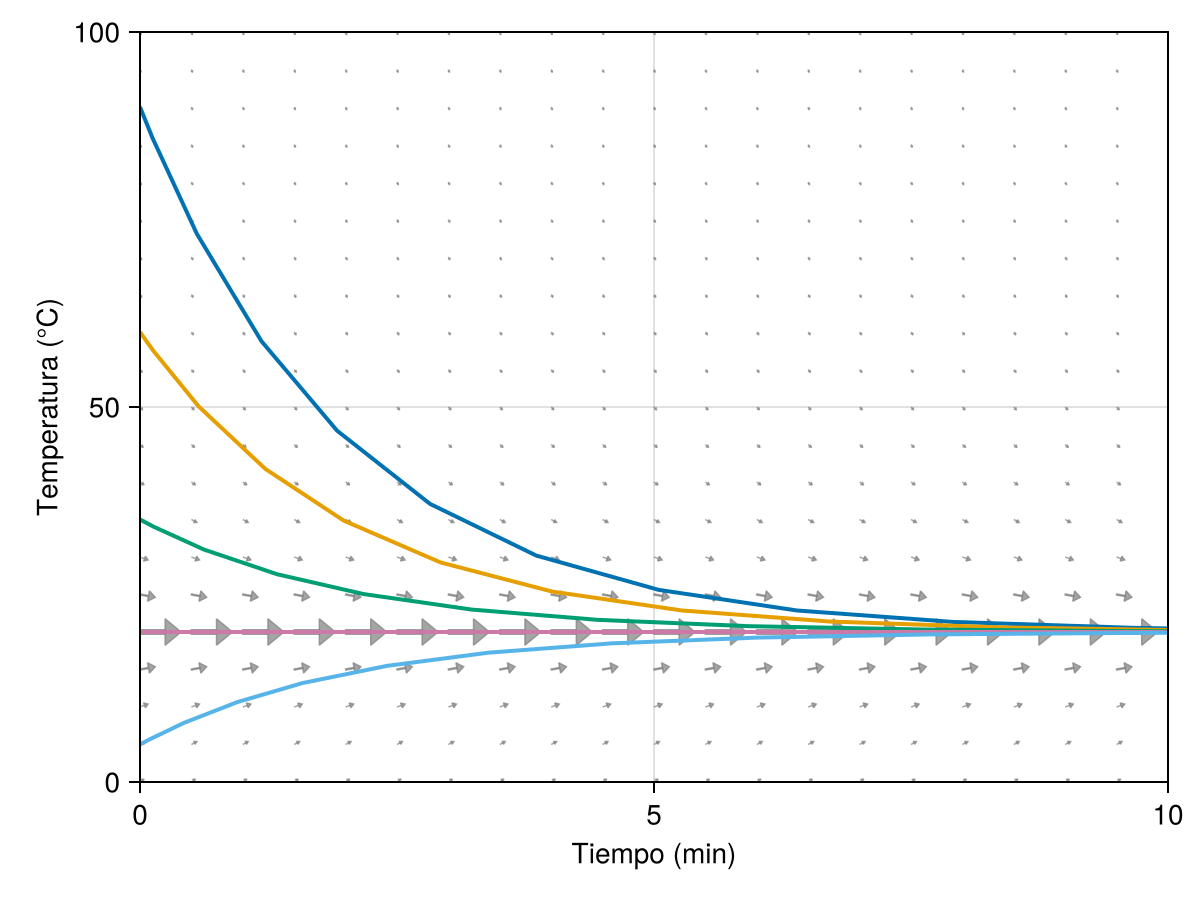
\includegraphics[keepaspectratio]{01-edos-primer-orden_files/figure-pdf/cell-11-output-2.png}}

  Todas las curvas integrales tienden a la temperatura ambiente
  \(y=20\): el campo de direcciones ``empuja'' cualquier solución hacia
  la recta horizontal \(y=20\), que es un punto de equilibrio estable.

  \end{tcolorbox}
\item
  Resolver simbólicamente la ecuación con la condición inicial
  \(y(0)=90\) y calcular cuánto tarda el café en alcanzar los \(30\) °C.

  \begin{tcolorbox}[enhanced jigsaw, arc=.35mm, bottomrule=.15mm, bottomtitle=1mm, breakable, colback=white, colbacktitle=quarto-callout-note-color!10!white, colframe=quarto-callout-note-color-frame, coltitle=black, left=2mm, leftrule=.75mm, opacityback=0, opacitybacktitle=0.6, rightrule=.15mm, title=\textcolor{quarto-callout-note-color}{\faInfo}\hspace{0.5em}{Ayuda}, titlerule=0mm, toprule=.15mm, toptitle=1mm]

  Usar la función
  \href{https://docs.juliahub.com/SymPyPythonCall/}{\texttt{dsolve}} del
  paquete \texttt{SymPyPythonCall} con el argumento \texttt{ics} para
  imponer la condición inicial, y la función \texttt{solve} para
  despejar el instante pedido.

  \end{tcolorbox}

  \begin{tcolorbox}[enhanced jigsaw, arc=.35mm, bottomrule=.15mm, bottomtitle=1mm, breakable, colback=white, colbacktitle=quarto-callout-tip-color!10!white, colframe=quarto-callout-tip-color-frame, coltitle=black, left=2mm, leftrule=.75mm, opacityback=0, opacitybacktitle=0.6, rightrule=.15mm, title=\textcolor{quarto-callout-tip-color}{\faLightbulb}\hspace{0.5em}{Solución}, titlerule=0mm, toprule=.15mm, toptitle=1mm]

  La ecuación es lineal (y separable). Simbólicamente:

\begin{Shaded}
\begin{Highlighting}[]
\ImportTok{using} \BuiltInTok{SymPyPythonCall}
\PreprocessorTok{@syms}\NormalTok{ t }\FunctionTok{y}\NormalTok{()}
\NormalTok{eq }\OperatorTok{=} \FunctionTok{Eq}\NormalTok{(}\FunctionTok{diff}\NormalTok{(}\FunctionTok{y}\NormalTok{(t), t), }\OperatorTok{{-}}\FloatTok{1}\OperatorTok{//}\FloatTok{2} \OperatorTok{*}\NormalTok{ (}\FunctionTok{y}\NormalTok{(t) }\OperatorTok{{-}} \FloatTok{20}\NormalTok{))}
\NormalTok{sol }\OperatorTok{=} \FunctionTok{dsolve}\NormalTok{(eq, }\FunctionTok{y}\NormalTok{(t), ics }\OperatorTok{=} \FunctionTok{Dict}\NormalTok{(}\FunctionTok{y}\NormalTok{(}\FloatTok{0}\NormalTok{) }\OperatorTok{=\textgreater{}} \FloatTok{90}\NormalTok{))}
\end{Highlighting}
\end{Shaded}

  $y{\left(t \right)} = 20 + 70 e^{- \frac{t}{2}}$

  Es decir, \(y(t) = 20 + 70e^{-t/2}\). El instante en que \(y(t)=30\):

\begin{Shaded}
\begin{Highlighting}[]
\NormalTok{t30 }\OperatorTok{=} \FunctionTok{solve}\NormalTok{(}\FunctionTok{Eq}\NormalTok{(}\FunctionTok{rhs}\NormalTok{(sol), }\FloatTok{30}\NormalTok{), t)[}\FloatTok{1}\NormalTok{]}
\FunctionTok{N}\NormalTok{(t30)}
\end{Highlighting}
\end{Shaded}

\begin{verbatim}
3.8918202981106265
\end{verbatim}

  El café alcanza los 30 °C a los \(2\ln 7 \approx 3.89\) minutos.

  \end{tcolorbox}
\end{enumerate}

\end{exercise}

\begin{exercise}[]\protect\hypertarget{exr-trayectorias-ortogonales}{}\label{exr-trayectorias-ortogonales}

\textbf{Aplicación geométrica: trayectorias ortogonales.} En
electrostática, las líneas de campo de una carga puntual son ortogonales
a las curvas equipotenciales. Las equipotenciales de un dipolo
bidimensional simplificado forman la familia de circunferencias

\[
x^2 + y^2 = 2Cx.
\]

Hallar la familia de trayectorias ortogonales (las líneas de campo) y
dibujar ambas familias.

\begin{tcolorbox}[enhanced jigsaw, arc=.35mm, bottomrule=.15mm, bottomtitle=1mm, breakable, colback=white, colbacktitle=quarto-callout-note-color!10!white, colframe=quarto-callout-note-color-frame, coltitle=black, left=2mm, leftrule=.75mm, opacityback=0, opacitybacktitle=0.6, rightrule=.15mm, title=\textcolor{quarto-callout-note-color}{\faInfo}\hspace{0.5em}{Ayuda}, titlerule=0mm, toprule=.15mm, toptitle=1mm]

Derivar implícitamente la familia y eliminar la constante \(C\) para
obtener la EDO \(y' = f(x,y)\) de la familia. La familia ortogonal
satisface \(y' = -1/f(x,y)\). La ecuación resultante es homogénea.

\end{tcolorbox}

\begin{tcolorbox}[enhanced jigsaw, arc=.35mm, bottomrule=.15mm, bottomtitle=1mm, breakable, colback=white, colbacktitle=quarto-callout-tip-color!10!white, colframe=quarto-callout-tip-color-frame, coltitle=black, left=2mm, leftrule=.75mm, opacityback=0, opacitybacktitle=0.6, rightrule=.15mm, title=\textcolor{quarto-callout-tip-color}{\faLightbulb}\hspace{0.5em}{Solución}, titlerule=0mm, toprule=.15mm, toptitle=1mm]

De \(x^2+y^2 = 2Cx\) se obtiene \(C = \frac{x^2+y^2}{2x}\), y derivando
implícitamente, \(2x + 2yy' = 2C\), luego

\[
y' = \frac{y^2 - x^2}{2xy}.
\]

La familia ortogonal satisface la ecuación homogénea
\(y' = \dfrac{2xy}{x^2 - y^2}\):

\begin{Shaded}
\begin{Highlighting}[]
\PreprocessorTok{@syms}\NormalTok{ x }\FunctionTok{y}\NormalTok{()}
\NormalTok{sol }\OperatorTok{=} \FunctionTok{dsolve}\NormalTok{(}\FunctionTok{Eq}\NormalTok{(}\FunctionTok{diff}\NormalTok{(}\FunctionTok{y}\NormalTok{(x), x), }\FloatTok{2}\NormalTok{x }\OperatorTok{*} \FunctionTok{y}\NormalTok{(x) }\OperatorTok{/}\NormalTok{ (x}\OperatorTok{\^{}}\FloatTok{2} \OperatorTok{{-}} \FunctionTok{y}\NormalTok{(x)}\OperatorTok{\^{}}\FloatTok{2}\NormalTok{)), }\FunctionTok{y}\NormalTok{(x))}
\end{Highlighting}
\end{Shaded}

$\left[\begin{smallmatrix}y{\left(x \right)} = - \frac{\sqrt{- 4 x^{2} + e^{2 C_{1}}}}{2} + \frac{e^{C_{1}}}{2}\\y{\left(x \right)} = \frac{\sqrt{- 4 x^{2} + e^{2 C_{1}}}}{2} + \frac{e^{C_{1}}}{2}\end{smallmatrix}\right]$

Reordenando la solución implícita se obtiene \(x^2 + y^2 = 2Ky\): las
líneas de campo son \textbf{circunferencias centradas en el eje \(y\) y
que pasan por el origen}, ortogonales a las equipotenciales
(circunferencias centradas en el eje \(x\) por el origen). Dibujamos
ambas familias:

\begin{Shaded}
\begin{Highlighting}[]
\NormalTok{plt }\OperatorTok{=}\NormalTok{ Plots.}\FunctionTok{plot}\NormalTok{(aspect\_ratio }\OperatorTok{=} \OperatorTok{:}\NormalTok{equal, legend }\OperatorTok{=} \ConstantTok{false}\NormalTok{, xlab }\OperatorTok{=}\NormalTok{ L}\StringTok{"x"}\NormalTok{, ylab }\OperatorTok{=}\NormalTok{ L}\StringTok{"y"}\NormalTok{, xlims }\OperatorTok{=}\NormalTok{ (}\OperatorTok{{-}}\FloatTok{3}\NormalTok{, }\FloatTok{3}\NormalTok{), ylims }\OperatorTok{=}\NormalTok{ (}\OperatorTok{{-}}\FloatTok{3}\NormalTok{, }\FloatTok{3}\NormalTok{))}
\NormalTok{θ }\OperatorTok{=} \FunctionTok{range}\NormalTok{(}\FloatTok{0}\NormalTok{, }\FloatTok{2}\NormalTok{π, length }\OperatorTok{=} \FloatTok{200}\NormalTok{)}
\ControlFlowTok{for}\NormalTok{ c }\KeywordTok{in}\NormalTok{ [}\FloatTok{0.5}\NormalTok{, }\FloatTok{1}\NormalTok{, }\FloatTok{1.5}\NormalTok{]}
\NormalTok{    Plots.}\FunctionTok{plot!}\NormalTok{(plt, c }\OperatorTok{.+}\NormalTok{ c }\OperatorTok{.*} \FunctionTok{cos}\NormalTok{.(θ),  c }\OperatorTok{.*} \FunctionTok{sin}\NormalTok{.(θ), color }\OperatorTok{=} \OperatorTok{:}\NormalTok{blue)   }\CommentTok{\# Equipotenciales}
\NormalTok{    Plots.}\FunctionTok{plot!}\NormalTok{(plt, }\OperatorTok{{-}}\NormalTok{c }\OperatorTok{.+}\NormalTok{ c }\OperatorTok{.*} \FunctionTok{cos}\NormalTok{.(θ), c }\OperatorTok{.*} \FunctionTok{sin}\NormalTok{.(θ), color }\OperatorTok{=} \OperatorTok{:}\NormalTok{blue)}
\NormalTok{    Plots.}\FunctionTok{plot!}\NormalTok{(plt, c }\OperatorTok{.*} \FunctionTok{cos}\NormalTok{.(θ),  c }\OperatorTok{.+}\NormalTok{ c }\OperatorTok{.*} \FunctionTok{sin}\NormalTok{.(θ), color }\OperatorTok{=} \OperatorTok{:}\NormalTok{red)    }\CommentTok{\# Líneas de campo}
\NormalTok{    Plots.}\FunctionTok{plot!}\NormalTok{(plt, c }\OperatorTok{.*} \FunctionTok{cos}\NormalTok{.(θ), }\OperatorTok{{-}}\NormalTok{c }\OperatorTok{.+}\NormalTok{ c }\OperatorTok{.*} \FunctionTok{sin}\NormalTok{.(θ), color }\OperatorTok{=} \OperatorTok{:}\NormalTok{red)}
\ControlFlowTok{end}
\NormalTok{plt}
\end{Highlighting}
\end{Shaded}

\pandocbounded{
\includegraphics[keepaspectratio]{index_files/mediabag/01-edos-primer-orden_files/figure-pdf/cell-15-output-1.pdf}}

En cada intersección, una circunferencia azul y una roja se cortan en
ángulo recto.

\end{tcolorbox}

\end{exercise}

\section{Ejercicios propuestos}\label{ejercicios-propuestos}

\begin{exercise}[]\protect\hypertarget{exr-propuesto-forense}{}\label{exr-propuesto-forense}

\textbf{Medicina forense.} Un cadáver se encuentra a 30 °C en una
habitación a 21 °C; una hora más tarde su temperatura es de 28 °C.
Suponiendo la ley de enfriamiento de Newton y temperatura corporal
normal de 36.5 °C, estimar la hora de la muerte.

\end{exercise}

\begin{exercise}[]\protect\hypertarget{exr-propuesto-mezclas}{}\label{exr-propuesto-mezclas}

\textbf{Ingeniería química.} Un tanque contiene 500 L de salmuera con 5
kg de sal. Entra agua con 0.02 kg/L de sal a 10 L/min y la mezcla sale
al mismo ritmo. Plantear y resolver la EDO de la cantidad de sal
\(y(t)\), y calcular la concentración a largo plazo.

\end{exercise}

\begin{exercise}[]\protect\hypertarget{exr-propuesto-hipoteca}{}\label{exr-propuesto-hipoteca}

\textbf{Finanzas.} Una hipoteca de 250 000 € a tipo continuo del 3.5 \%
se amortiza con pagos continuos de \(p\) €/año: \(D' = 0.035D - p\).
Calcular el pago \(p\) necesario para cancelar la deuda en 25 años y el
interés total pagado.

\end{exercise}

\begin{exercise}[]\protect\hypertarget{exr-propuesto-paracaidista}{}\label{exr-propuesto-paracaidista}

\textbf{Física.} Un paracaidista de 80 kg cae con rozamiento
proporcional al cuadrado de la velocidad, \(mv' = mg - kv^2\) con
\(k=0.27\) kg/m. Calcular la velocidad límite, resolver la ecuación
(separable) y dibujar la línea de fases.

\end{exercise}

\begin{exercise}[]\protect\hypertarget{exr-propuesto-bifurcacion}{}\label{exr-propuesto-bifurcacion}

\textbf{Ecología.} Estudiar las bifurcaciones del modelo de un insecto
plaga \(y' = ry\left(1-\frac{y}{K}\right) - \frac{y^2}{1+y^2}\) con
\(K=10\) fijo, en función de \(r>0\), localizando numéricamente los
valores de \(r\) donde cambia el número de equilibrios.

\end{exercise}




\end{document}
